\documentclass{beamer}
\usetheme{Madrid} % My favorite!
\setbeamercovered{invisible}
\usefonttheme{serif}
% To remove the navigation symbols from 
% the bottom of slides%
\setbeamertemplate{navigation symbols}{} 
% 
\usepackage{graphicx}
% 
\title[Online Social Network Privacy]{A Framework for Computing the
  Privacy Scores of Users in Online Social Networks}
%\author{Kun Liu}

\date{\today}
\begin{document}
% Title page of this presentation. 
\begin{frame}
  \titlepage
\end{frame}

% problem and contribution. 
\begin{frame}
  \frametitle{Problem Description}
  \begin{block}
    {How to measure privacy risk of social network users?}
    \begin{itemize}
      \LARGE{
    \item Privacy protection Related works. 
      \begin{itemize}
        \Large{
      \item Spamming and Phishing.
      \item Social network Attacks. 
      \item Access control privacy control.
      \item Multi-party collaborative privacy control. 
      \item ...}
      \end{itemize}
    \item How to evaluate the risk level? }
    \end{itemize}
  \end{block}
\end{frame}

% Contribution of this paper.
\begin{frame}
  \frametitle{Contributions of This Paper}
    \begin{itemize} 
      \LARGE{
      \item A privacy score computation model. 
      \item Model validation method. }
    \end{itemize}
\end{frame}

\begin{frame}%[fragile] % Notice the [fragile] option %
  \frametitle{General Observations and Intuitions}
  \begin{itemize}
    \LARGE{
    \item Different profile items have different contribution to
      privacy score. 
    \item The visibility of information can affect the privacy score.}
  \end{itemize}
\end{frame}

% Modelling online social network profile settings. 
\begin{frame}[fragile]
  \frametitle{Modeling Social Network Users}

  \begin{figure}
    \begin{center}
      
\includegraphics[scale=1.5]{socialnetwork}
    \end{center}
  \end{figure}

\[
\Longrightarrow
 R_{n,N} =
 \begin{pmatrix}
  R_{1,1} & R_{1,2} & \cdots & R_{1,N} \\
  R_{2,1} & R_{2,2} & \cdots & R_{2,N} \\
  \vdots  & \vdots  & \ddots & \vdots  \\
  R_{n,1} & R_{n,2} & \cdots & R_{n,N}
 \end{pmatrix}
\]

\end{frame}

% IRT model description.
\begin{frame}[fragile]
  \frametitle{The Item Response Theory(IRT) Model}
\Huge{
  \[P_{ij}=\frac{1}{1+e^{-\alpha_i(\theta_j-\beta_i)}}\]
}
\end{frame}

% IRT based Privacy score model. 
% \begin{frame}
%   \frametitle{IRT based Privacy Score model.}
%   We can use IRT to model the privacy score estimation. But we need to
%   reinterpret the IRT model as follows. \\ 
%   \begin{enumerate}
%     \item Examinee mapped to a user and question mapped to profile
%       item. 
%     \item The ability of examinee $\theta_j$ corresponses to attitude of
%       user $j$. 
%     \item The difficulty $\beta_i$ corresponses to
%       \textit{sensitivity} of of profile item $i$. 
%     \item Question discrimination parameter $\alpha_i$ is ignored, and
%       it can be used to adjust the analysis of items and users. 
%   \end{enumerate}
% \end{frame}

% privacy score definition.
\begin{frame}[fragile]
  \frametitle{Definition of the Privacy Score}
  % Intuitively, the privacy score should be monotonically increasing with
  % both sensitivity and visibility. So, this paper defines privacy
  % score of user $j$ for item $i$ as \textsc{Pr}$(i,j)=\beta_i\times
  % V(i,j)$, and by summing up all the item privacy for user $j$, we get
  % the privacy score for user $j$ as
\begin{align}
  \textsc{Pr}(i,j)=\beta_i\times V(i,j) \\
  \textsc{Pr}(j)=\sum_{i=1}^{n}\textsc{Pr}(i,j)=\sum_{i=1}^n\beta_i\times
  V(i,j). \\
  V(i,j)=P_{ij}\times 1 + (1-P_{ij})\times 0 = P_{ij}
\end{align}
  where \[P_{ij} = Prob\{\textbf{R}(i,j)=1\}.\]
  \Large{\textbf{GOAL:} $\beta_i$ and $V(i,j)$}.
\end{frame}

% Estimating sensitivity with MLE. 
\begin{frame}
  \frametitle{\large{Estimating sensitivity $\xi_i=(\alpha_i,\beta_i)$ when
      $\overrightarrow{\theta}=(\theta_1,\dots,\theta_N)$ is known.}}
      \Large{Use Maximum Likelihood Estimation(MLE).}
      \large{
        % \begin{eqnarray}
        %   10xy^2+15x^2y-5xy & = & 5\left(2xy^2+3x^2y-xy\right) \nonumber \\
        %   & = & 5x\left(2y^2+3xy-y\right) \nonumber \\
        %   & = & 5xy\left(2y+3x-1\right)
        % \end{eqnarray}
        \begin{eqnarray}
          \xi_i^{MLE}&=&\underset{\xi}{\operatorname{\arg\max}}
          {\prod_{j=1}^NP_{ij}^{R(i,j)}(1-P_{ij})^{1-R(i,j)}}
          \nonumber \\
          &=& \underset{\xi}{\operatorname{\arg\max}}
          {\sum_{j=1}^NR(i,j) log(P_{ij})+(1-R(i,j))log(1-P_{ij})}
          \nonumber \\
          &=&\underset{\xi}{\operatorname{\arg\max}}
          {\sum_{g=1}^K[r_{ig}logP_i(\theta_g)+(f_g-r_{ig})log(1-P_i(\theta_g))]}
        \end{eqnarray}
        }
      % By Partitioning social network users $\{1,\dots,N\}$ into $K$
      % non-overlapping groups $\{F_1,\ldots,F_K\}$ s.t. $\cup_{g=1}^KF_g=\{1,\ldots,N\}$. \\ 
      % We can derive log-likelihood function as : 
      % \[\xi_i^{MLE}=\underset{\xi}{\operatorname{\arg\max}}
      % {\sum_{g=1}^K[r_{ig}logP_i(\theta_g)+(f_g-r_{ig})log(1-P_i(\theta_g))]}\]
\end{frame}

% Estimating sensitivity with EM method.
\begin{frame}
  \frametitle{\small{Estimating sensitivity $\xi_i=(\alpha_i,\beta_i)$ when
      $\overrightarrow{\theta}=(\theta_1,\dots,\theta_N)$ is unknown.}}
  \begin{block}
      {Use Expectation Maximization (EM) method.}
      \textbf{E-Step:} Compute $E[f_g]$ and $E[r_{ig}]$ as follows:

      \[E[f_g]=\overline{f_g}=\sum_{j=1}^NP(\theta_g|R^j,\overrightarrow{\xi})\] 
      \[E[r_{ig}]=\overline{r_{ig}}=\sum_{j=1}^NP(\theta_g|R^j,\overrightarrow{\xi}\times R(i,j)).\]
      %$P(\theta_g|R^j,\overrightarrow{\xi})$ denote the posterior probability
      %distribution of a user's attitude. 

      \textbf{M-Step:} Estimate $\overrightarrow{\xi}$ with the values
      of $\overline{f_g}$ and $\overline{r_{ig}}$.
  \end{block}
\end{frame}

% posterior probability calculation. 
\begin{frame}
  \frametitle{Calculating the Posterior Probability of Attitudes}
  \[P(\theta_j|R^j,\overrightarrow{\xi})=\frac{P(R^j|\theta_j,\overrightarrow{\xi})g(\theta_j)}
  {\int{P(R^j|\theta_j,\overrightarrow{\xi})g(\theta_j)d\theta_j}}\]
  By partitioning user attitude into different groups, we can transform the $\int$
  to $\sum$ as show below: 
  \[P(\theta_j|R^j,\overrightarrow{\xi})=\frac{P(R^j|X_t,\overrightarrow{\xi})g(X_t)}
  {\sum_{t=1}^K{P(R^j|X_t,\overrightarrow{\xi})g(X_t)}}\]
  In this formula, $K$ is the number of groups of user attitudes, and user
  attitudes are partitioned into points $\{X_1,X_2,\ldots,X_K\}$. $A(X_t)$ is
  the attribute probability value determined by $X_t$ and $\sum_{t=1}^KA(X_t)=1$.
\end{frame}

% 
\begin{frame}
  \frametitle{Computation of Visibility}
  Estimating $\overrightarrow{\theta}$ by:
  \[\overrightarrow{\theta^{MLE}}=\underset{\xi}{\operatorname{\arg\max}}
  {\sum_{i=1}^n[R(i,j)logP_{ij}+(1-R(i,j))log(1-P_{ij})]}\]
  And then, 
  \[V(i,j)=P_{ij}=Prob\{R(i,j)=1\}=\frac{1}{1+e^{-\alpha_i(\theta_j-\beta_i)}}\]
\end{frame}

% \begin{frame}
%   \frametitle{Polytomous Privacy score computation}
%   The above dichotomous privacy model can be easily promoted to the one with
%   multiple privacy settings. (Omitted currently)
% \end{frame}

% 
\begin{frame}
  %\frametitle{Finally, we can compute the privacy score use IRT method}
  \frametitle{A naive privacy score computation method}

  \textbf{Naive computation of Sensitivity:}
  \[\beta_i=\frac{N-|R_i|}{N}\] 
  $|R_i|$ is the number of users who set item $i$ as visible. %or 
  %\[\beta_{ik}^*=\frac{N-\sum_{j=1}^NI_{R(i,j)\leq k}}{N}\] for polychotomous case. 

  \textbf{Naive computation of Visibility:}
  \[P_{ij}=\frac{|R_i|}{N}\times \frac{|R^j|}{n}\]% and 
  % \[P_{ijk}=\frac{\sum_{j=1}^NI_{(R(i,j)=k)}}{N}\times
  % \frac{\sum_{i=1}^nI_{R(i,j)=k}}{n}\]
  % for polychotomous case. 
\end{frame}

\begin{frame}
  \frametitle{Experiment results}
  \begin{figure}
    \begin{center}
    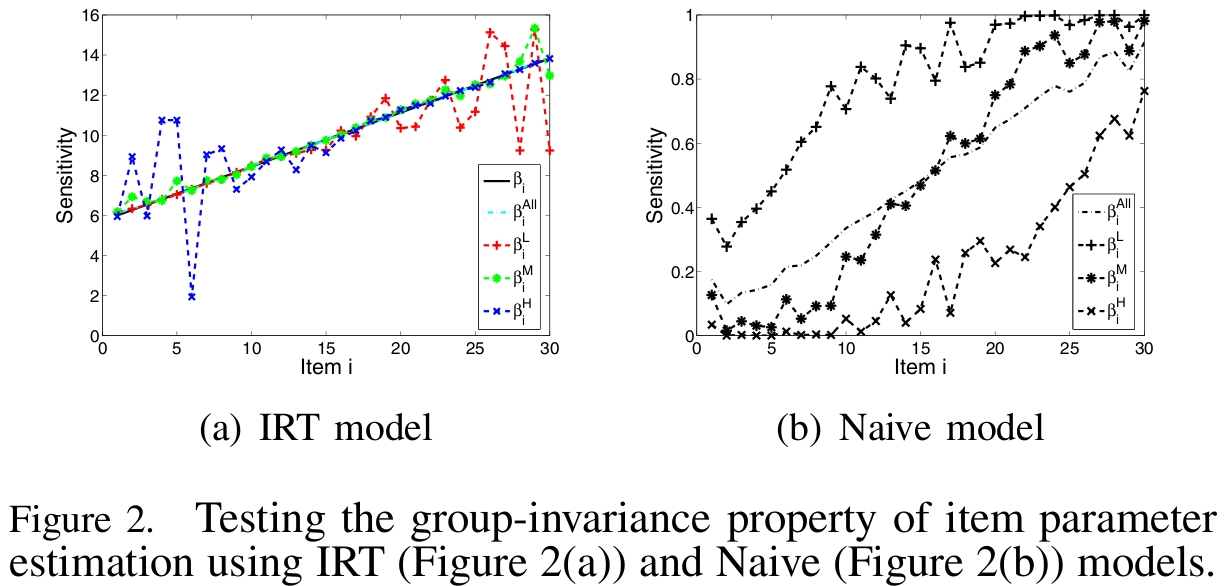
\includegraphics[scale=0.25]{result}
  \end{center}
  \end{figure}
\end{frame}

\begin{frame}
  \frametitle{Weakness of this paper}
  \begin{enumerate}
    \item This paper fails to explicitely consider the effects of
      social graph. 
    \item This paper doesn't consider the balance between privacy and
      utility. Utility here is not clearly defined. 
  \end{enumerate} 
\end{frame}

\begin{frame}
  \centerline{The End, Thanks!}
\end{frame}
% End of slides
\end{document}